\begin{figure}[!tp]
    \setlength{\abovecaptionskip}{4pt}
    \setlength{\belowcaptionskip}{-8pt}
    \centering
    % Row 1: appearance is scaled by ~1.16 to offset its y-axis label,
    % so all three plot areas render at the same size.
    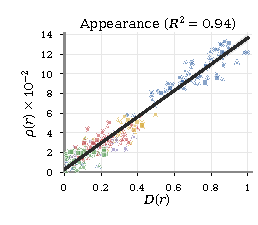
\includegraphics[width=0.348\columnwidth]{images/scatter_facet_appearance.pdf}\hfill
    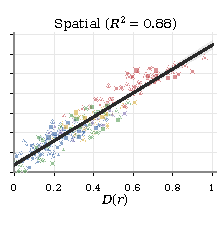
\includegraphics[width=0.300\columnwidth]{images/scatter_facet_spatial.pdf}\hfill
    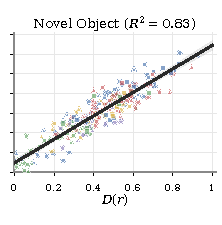
\includegraphics[width=0.300\columnwidth]{images/scatter_facet_novel.pdf}\\[3pt]
    % Row 2: two panels at the same plot-area size, centered
    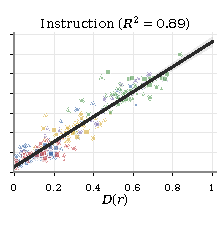
\includegraphics[width=0.300\columnwidth]{images/scatter_facet_instruction.pdf}\hspace{0.024\columnwidth}%
    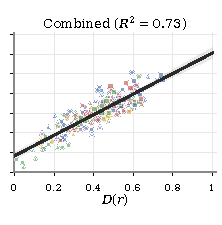
\includegraphics[width=0.300\columnwidth]{images/scatter_facet_combined.pdf}\\[3pt]
    % Legend
    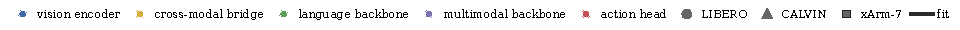
\includegraphics[width=\columnwidth]{images/scatter_facet_legend.pdf}
    \caption{Predicted score $D(r)$ against measured cost $\rho(r)$ by shift type. Each point is one region of one architecture, benchmark, and seed, colored by region role, and squares overlay the physical xArm-7 measurements with OpenVLA-OFT. The combined panel spans a narrower cost range, which lowers its per-panel $R^2$ but not the pooled $R^2 = 0.89$ (Table~\ref{tab:diagnostic-aggregate}).}
    \label{fig:diagnostic-scatter-facets}
\end{figure}